\section{Performance}
Abbiamo misurato le performance (in millisecondi) dei tre algoritmi utilizzando 68 grafi di diverse dimensioni.
I grafi testati hanno un numero di nodi che variavano dai  10 ai 100000.
Come già detto, per ogni dimensione sono presenti quattro grafi e, per ottenere una misurazione dei tempi più precisa, vengono calcolati e sommati i tempi per ogni grafo (della stessa dimensionalità) e il tempo medio viene calcolato dividendo questo risultato per il numero di grafi.

Nei risultati finali, per ogni algoritmo, avremo 1 risultato per ogni dimensionalità dei grafi. 
Per questo motivo, nel momento in cui viene calcolata la complessità teorica, come numero di archi vengono considerati la media degli archi per ogni dimensionalità. 

Inoltre per i grafi di piccola dimensione (numero\_nodi <= 100) il singolo grafo viene iterato più volte su un algoritmo in modo da ottenere un ulteriore precisione nella misurazione cronologica.

\subsection{Prim}
L'algoritmo di Prim ha una complessità teorica di $O(mlogn)$, perciò ci aspettiamo indicativamente lo stesso risultato anche nella sua applicazione.

\begin{figure}[htbp]
    \centering
    \centerline{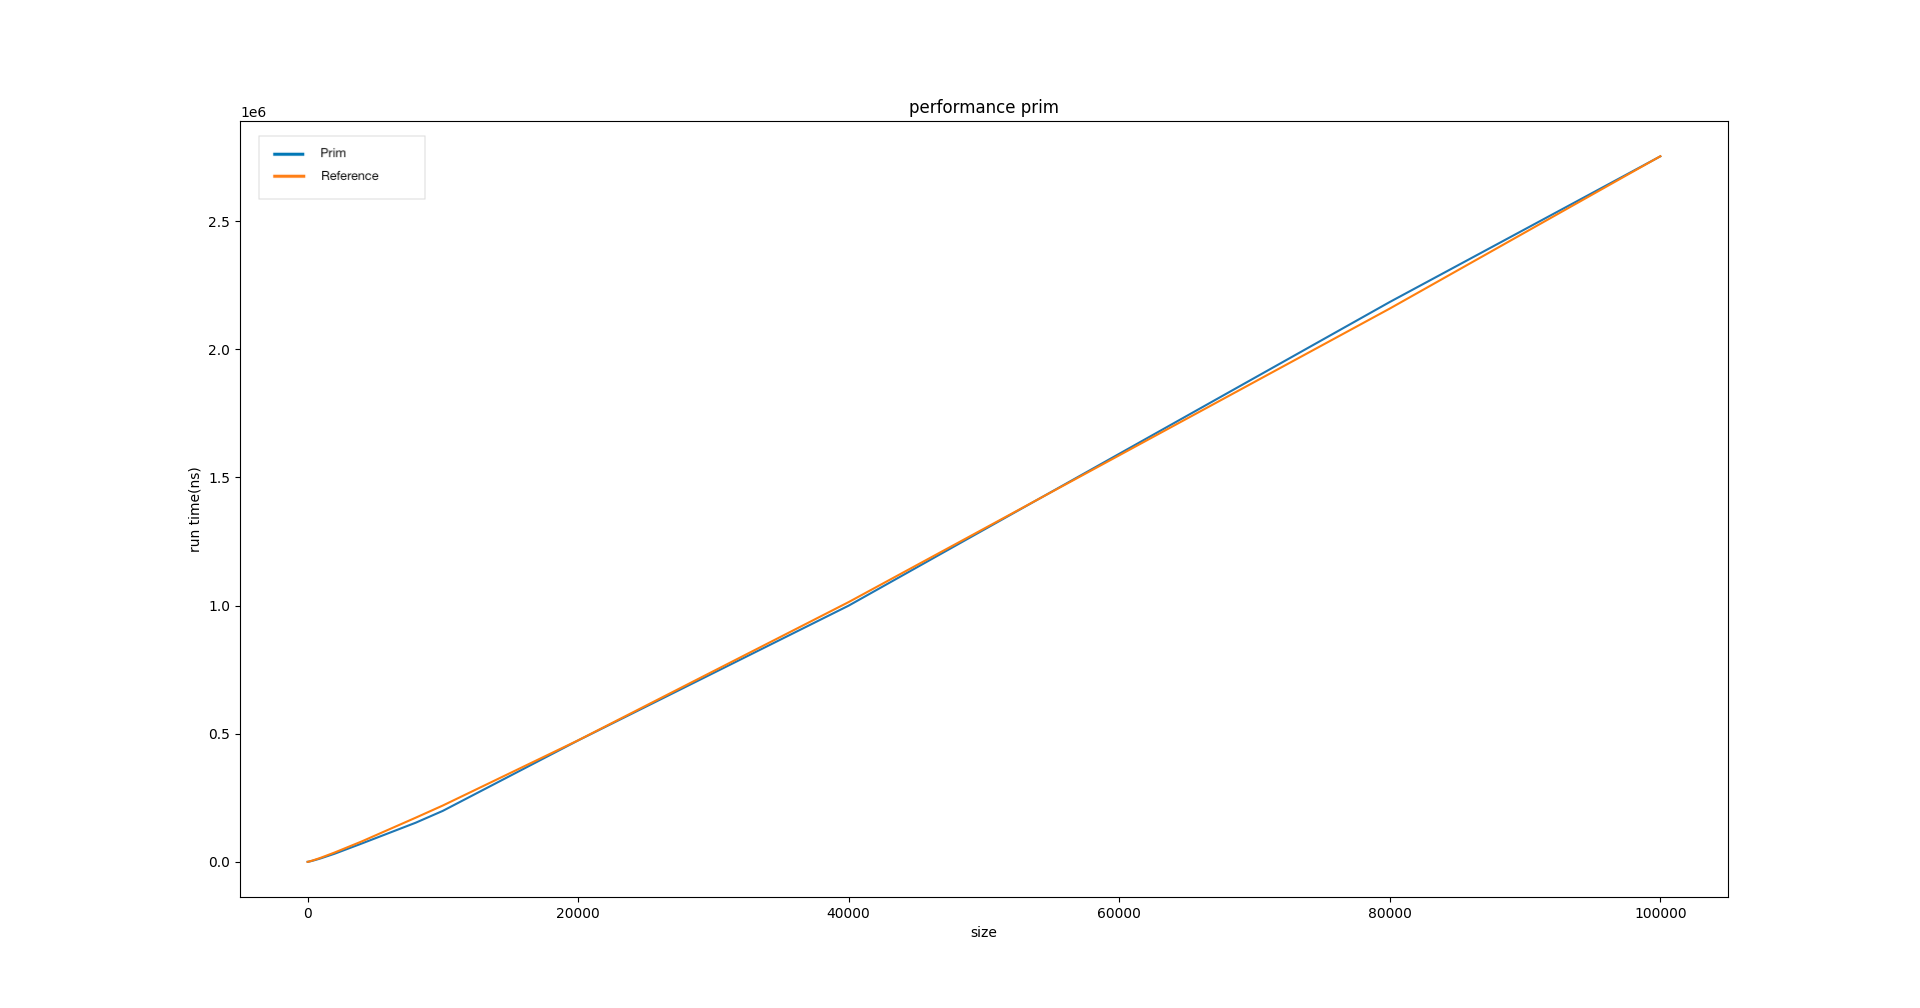
\includegraphics[scale = 0.38]{Fig/primFinale.png}}
    \caption{grafico dei tempi di Prim, in blu si ha il grafico con i tempi teorici moltiplicato per la costante e in arancio il grafico calcolato}
    \label{Prim}
\end{figure}



\subsection{Kruskal}
Anche kruskal, come Prim, ha una complessità di $O(mlogn)$

\begin{figure}[htbp]
    \centering
    \centerline{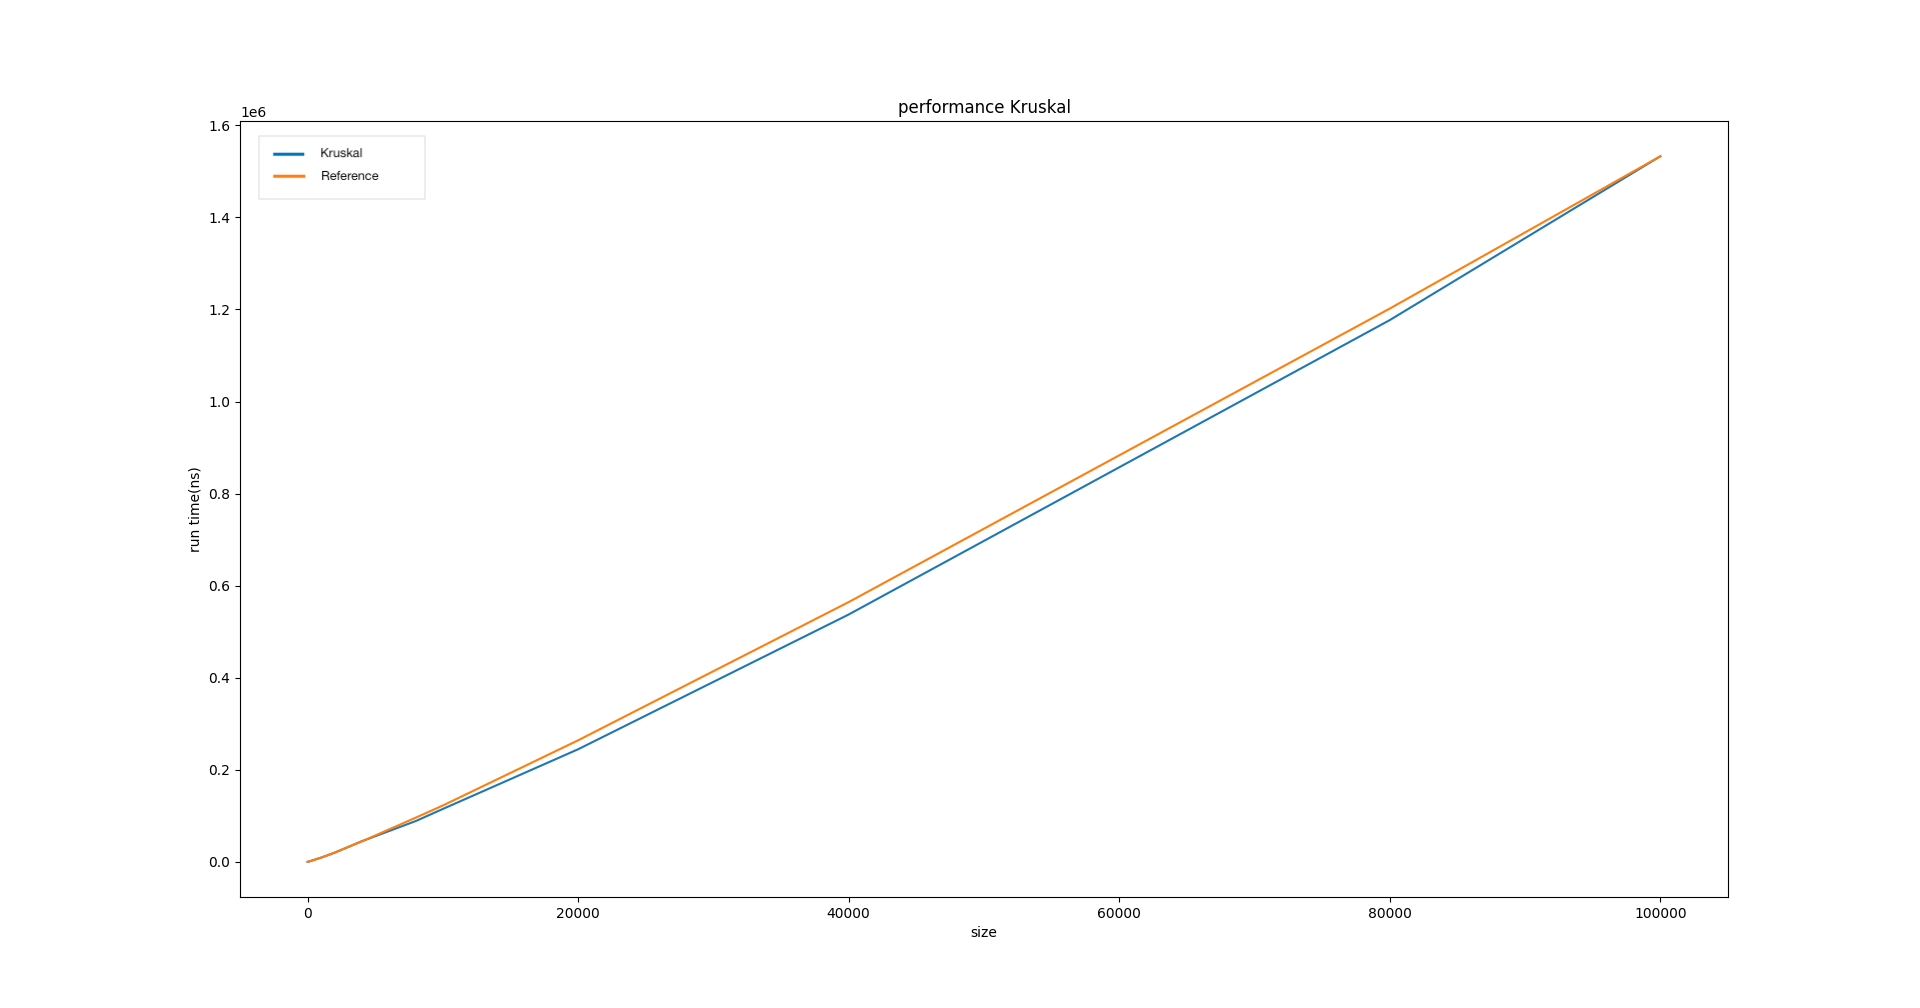
\includegraphics[scale = 0.38]{Fig/KruskalFinale.png}}
    \caption{grafico dei tempi di kruskal,  in blu si ha il grafico con i tempi teorici moltiplicato per la costante e in arancio il grafico calcolato}
    \label{Kruskal}
\end{figure}

\newpage
\subsection{Kruskal naive}
Per quanto riguarda la versione non ottimizzata dell'algoritmo di Kruskal, cioè quella che ad ogni iterazione del ciclo esegue una ricerca in profondità per assicurarsi che il nuovo arco non vada a creare cicli, ha una complessità di $O(mn)$.

Per la versione naive di Kruskal è stata fatta una piccola miglioria. L' algoritmo termina se:
\begin{itemize}
    \item sono stati scorsi tutti i lati del grafo
    \item è stato aggiunto al grafo di copertura minimo n-1 archi, in questo caso termina l'esecuzione.
\end{itemize}
Dato che la maggior parte dei grafi testati mediamente aveva un numero maggiore di archi rispetto al numero di nodi, grazie alla seconda condizione la costante nascosta all'interno dell'algoritmo si è abbassata. 

\begin{figure}[htbp]
    \centering
    \centerline{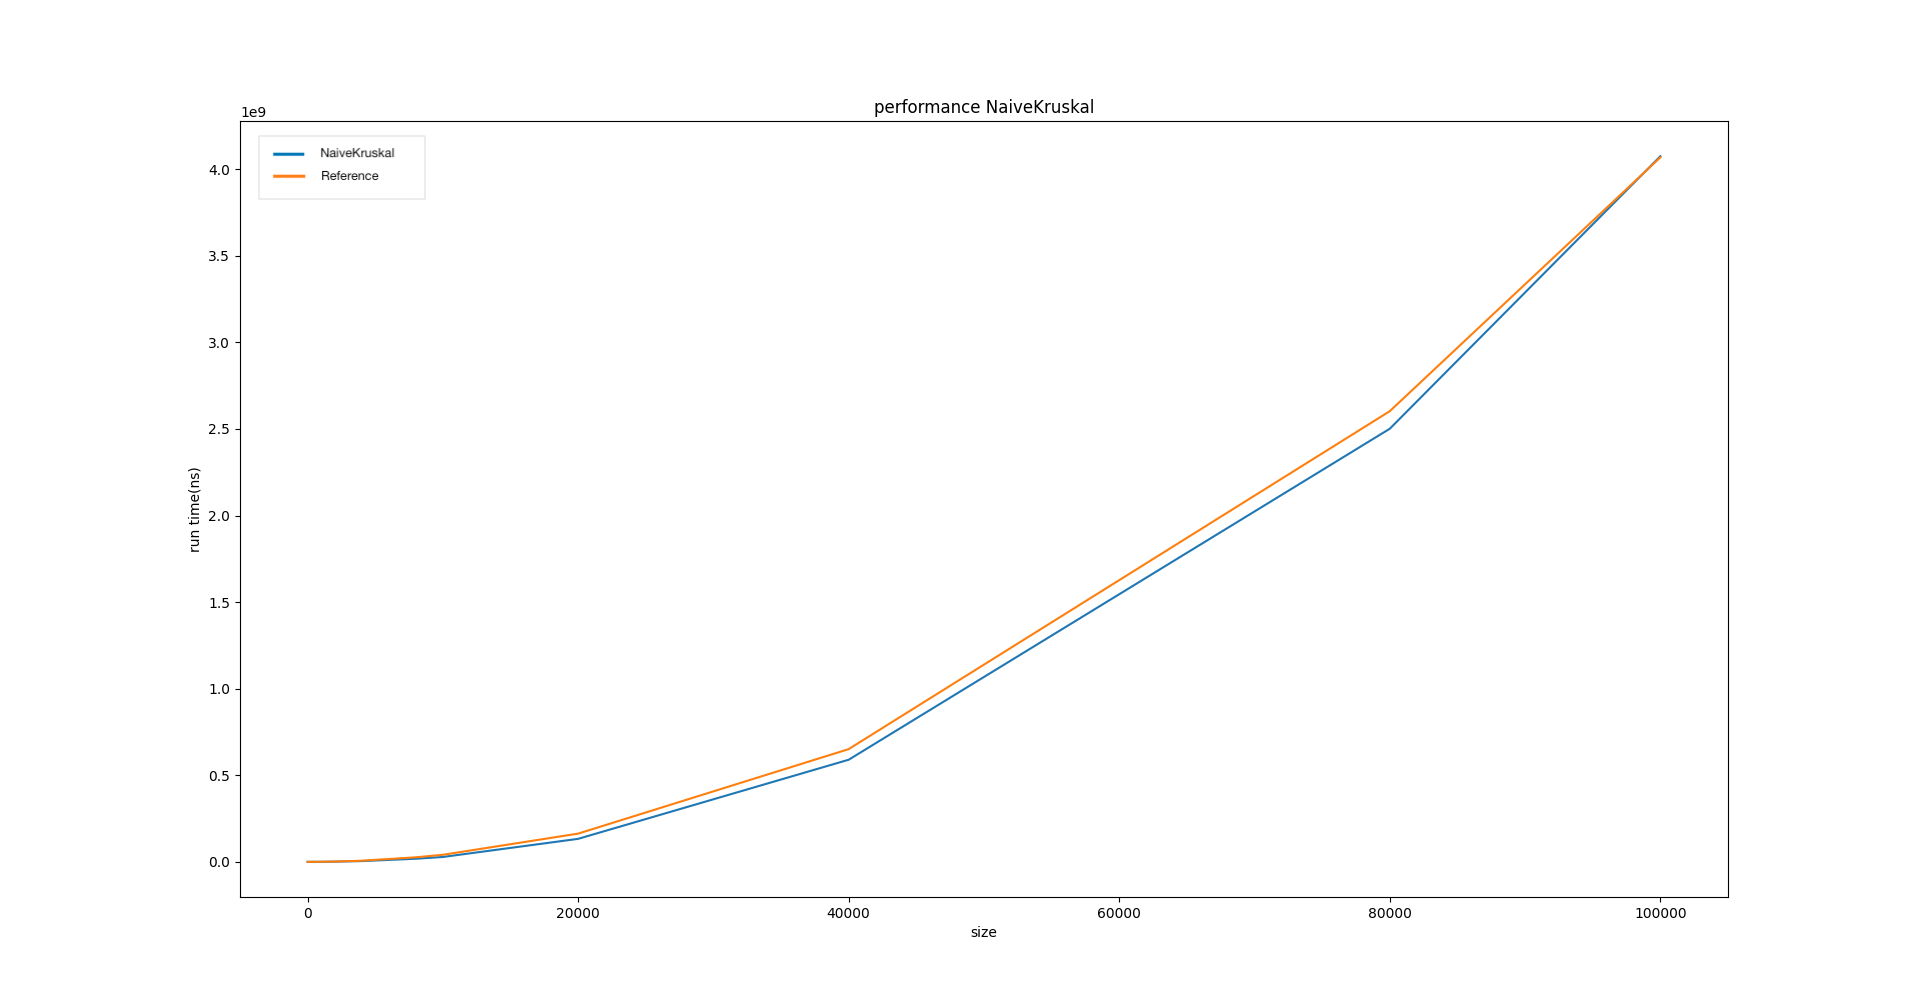
\includegraphics[scale = 0.38]{Fig/NaiveKruskalFinale.png}}
    \caption{grafico dei tempi di Kruskal naive, in blu si ha il grafico con i tempi teorici moltiplicato per la costante e in arancio il grafico calcolato}
    \label{Kruskal naive}
\end{figure}


Come si può notare dai grafici, la curva dei tempi di Prim, Kruskal e Kruskal naive (arancione) va quasi a sovrapporsi ai grafici teorici(blu) moltiplicati per la costante calcolata di ogni algoritmo, questo conferma che l'implementazione rispetta la complessità teorica degli algoritmi.

\newpage
\subsection{Risultati numerici}

Di seguito sono riportate le tabelle con i tempi utilizzati per la costruzione dei grafici sovrastanti. Nell'ordine Prim, Kruskal e KruskalNaive.

\rowcolors{2}{white!80!lightgray!90}{white}
\renewcommand{\arraystretch}{2}
\begin{longtable}[H]{|p{2cm}|p{2cm}|p{3cm}|p{3cm}|p{3cm}|} 
\hline

    \rowcolor{lightgray}
    \textbf{n\_nodi} & \textbf{times} & \textbf{costant} & \textbf{ratio}\\ \hline\hline  \endhead
    10	&	38.0	&		1.535	&	None \\ \hline
    20	&	100.0	&		1.309	&	2.632 \\ \hline
    40	&	260.0	&		1.355 &		2.6     \\ \hline
    80	&	619.0	&		1.329 &		2.381  \\ \hline
    100	&	835.0	&		1.358 &		1.349 \\ \hline
    200	&	2021.0	&		1.423 &		2.42 \\ \hline
    400	&	4741.0	&		1.492 &		2.346 \\ \hline
    800	&	10747.0	&		1.515 &		2.267 \\ \hline
    1000 &	14005.0	&		1.534 &		1.303 \\ \hline
    2000 &	31601.0	&		1.557 &		2.256 \\ \hline
    4000 &	71375.0	&	    1.61 &		2.259 \\ \hline
    8000 &	152772.0 &		1.589 &		2.14 \\ \hline
    10000 &	198903.0 &		1.623 &		1.302 \\ \hline
    20000 &	473662.0 &		1.791 &		2.381 \\ \hline
    40000 &	999872.0 &		1.768 &		2.111 \\ \hline
    80000 &	2184898.0 &		1.814 &		2.185 \\ \hline
    100000 &	2753401.0 &	1.793 &		1.26  \hline
    
    \caption{tabella riassuntiva di Prim}
\end{longtable}

\rowcolors{2}{white!80!lightgray!90}{white}
\renewcommand{\arraystretch}{2}
\begin{longtable}[H]{|p{2cm}|p{2cm}|p{3cm}|p{3cm}|p{3cm}|} \hline
    \rowcolor{lightgray}
    \textbf{n\_nodi} & \textbf{times} & \textbf{costant} & \textbf{ratio} \\ \hline\hline
    \endhead
    10	&	    46.0	&		1.858 &		None \\ \hline
    20	&	    113.0	&		1.479 &		2.457 \\ \hline
    40	&	    238.0	&		1.241 &		2.106 \\ \hline
    80	&	    522.0	&		1.121 &		2.193 \\ \hline
    100	&	    650.0	&		1.057 &		1.245 \\ \hline
    200	&	    1593.0	&		1.122 &		2.451 \\ \hline
    400	&	    3486.0	&		1.097 &		2.188 \\ \hline
    800	&	    7315.0	&		1.031 &		2.098 \\ \hline
    1000 &	    9082.0	&		0.995 &		1.242 \\ \hline
    2000 &	    19697.0	&		0.97  &  	2.169 \\ \hline
    4000 &	    44597.0	&	    1.006 &		2.264 \\ \hline
    8000 &		88609.0	&	    0.922 &		1.987 \\ \hline
    10000 &		114837.0 &		0.937 &		1.296 \\ \hline
    20000 &		244539.0 &		0.924 &		2.129 \\ \hline
    40000 &		537266.0 &		0.95 &		2.197 \\ \hline
    80000 &		1176867.0 &		0.977 &	    2.19 \\ \hline
    100000 &	1532773.0 &		0.998 &	    1.302 \hline
    \caption{tabella riassuntiva di Kruskal}
\end{longtable}

\newpage
\rowcolors{2}{white!80!lightgray!90}{white}
\renewcommand{\arraystretch}{2}
\begin{longtable}[H]{|p{2cm}|p{2cm}|p{3cm}|p{3cm}|p{3cm}|} \hline
    \rowcolor{lightgray}
    \textbf{n\_nodi} & \textbf{times} & \textbf{costant} & \textbf{ratio} \\ \hline\hline
    \endhead
    10	&	72.0		&	0.67	&	None \\ \hline
    20	&	238.0		&	0.467	&	3.306 \\ \hline
    40	&	583.0		&	0.28 &		2.45 \\ \hline
    80	&	2485.0		&	0.292 &		4.262 \\ \hline
    100	&	3034.0		&	0.227   &	1.221 \\ \hline
    200	&	11917.0		&	0.222	&	3.928 \\ \hline
    400	&	42721.0		&	0.201	&	3.585 \\ \hline
    800	&	166700.0	&	0.196	&   3.902 \\ \hline
    1000 &	262169.0	&	0.198	&   1.573 \\ \hline
    2000 &	1099545.0	&	0.206	&   4.194 \\ \hline
    4000 &	4371607.0	&	0.204 &		3.976 \\ \hline
    8000 &	17944643.0	&	0.21 &		4.105 \\ \hline
    10000 &	28077773.0	&	0.211 &		1.565 \\ \hline
    20000 &	132740246.0	&	0.248 &		4.728 \\ \hline
    40000 &	589607712.0	&	0.276 &		4.442 \\ \hline
    80000 &	2501403023.0 &	0.293 &		4.242 \\ \hline
    100000 &	4075177518.0 &	0.305 &		1.629  \hline
    \caption{tabella riassuntiva di Kruskal naive}
\end{longtable}

Come si può notare dalle tabelle che riassumono i risultati per ogni algoritmo, anche il ratio calcolato corrisponde a quello voluto. Infatti per quanto riguarda il ratio di Prim e Kruskal ($\sim 2,2$) \footnote{il ratio considerato, così come la costante per calcolare il grafico teorica, è quello corrispondente all'ultima istanza (100000)} sono quasi equivalenti e corrispondono al ratio teorico $2m*log(2n) / m*log(n)$.
Equivalentemente lo stesso discorso vale per Kruskal naive dove il ratio (4,4) corrisponde a circa il ratio teorico $2m*2n/m*n$


